%Texlive-full Version 3.141592-1.40.3 (Web2C 7.5.6)
%Kile Version 2.0.83
%File associated : SoFa_Logo.ps , FF.ps

\documentclass[a4paper,10pt]{article}
\usepackage[utf8x]{inputenc}
\usepackage[T1]{fontenc} 

\usepackage{lmodern}
\usepackage[a4paper]{geometry}
%\usepackage[frenchb]{babel}
\usepackage{graphicx}
\usepackage{hyperref}

\usepackage{pstricks}
\usepackage{pst-node}
%\usepackage{wrapfig}
\usepackage{amsmath}
\usepackage{amsfonts}
\usepackage{amssymb}
\usepackage{textcomp}
%\usepackage{mathaccent}
\usepackage{listings}
\lstset{language=C++,basicstyle=\scriptsize \color{green},identifierstyle=\color{orange},keywordstyle=[1]\color{blue},columns=fullflexible,commentstyle=\textit}

\usepackage{color}



\begin{document}
%%%%%%%%%%%%%%%%%%   LOGO  %%%%%%%%%%%%%%%%%%%%%%%%%
\begin{center}
\rput(6,1.5){\href{http://www.sofa-framework.org/}{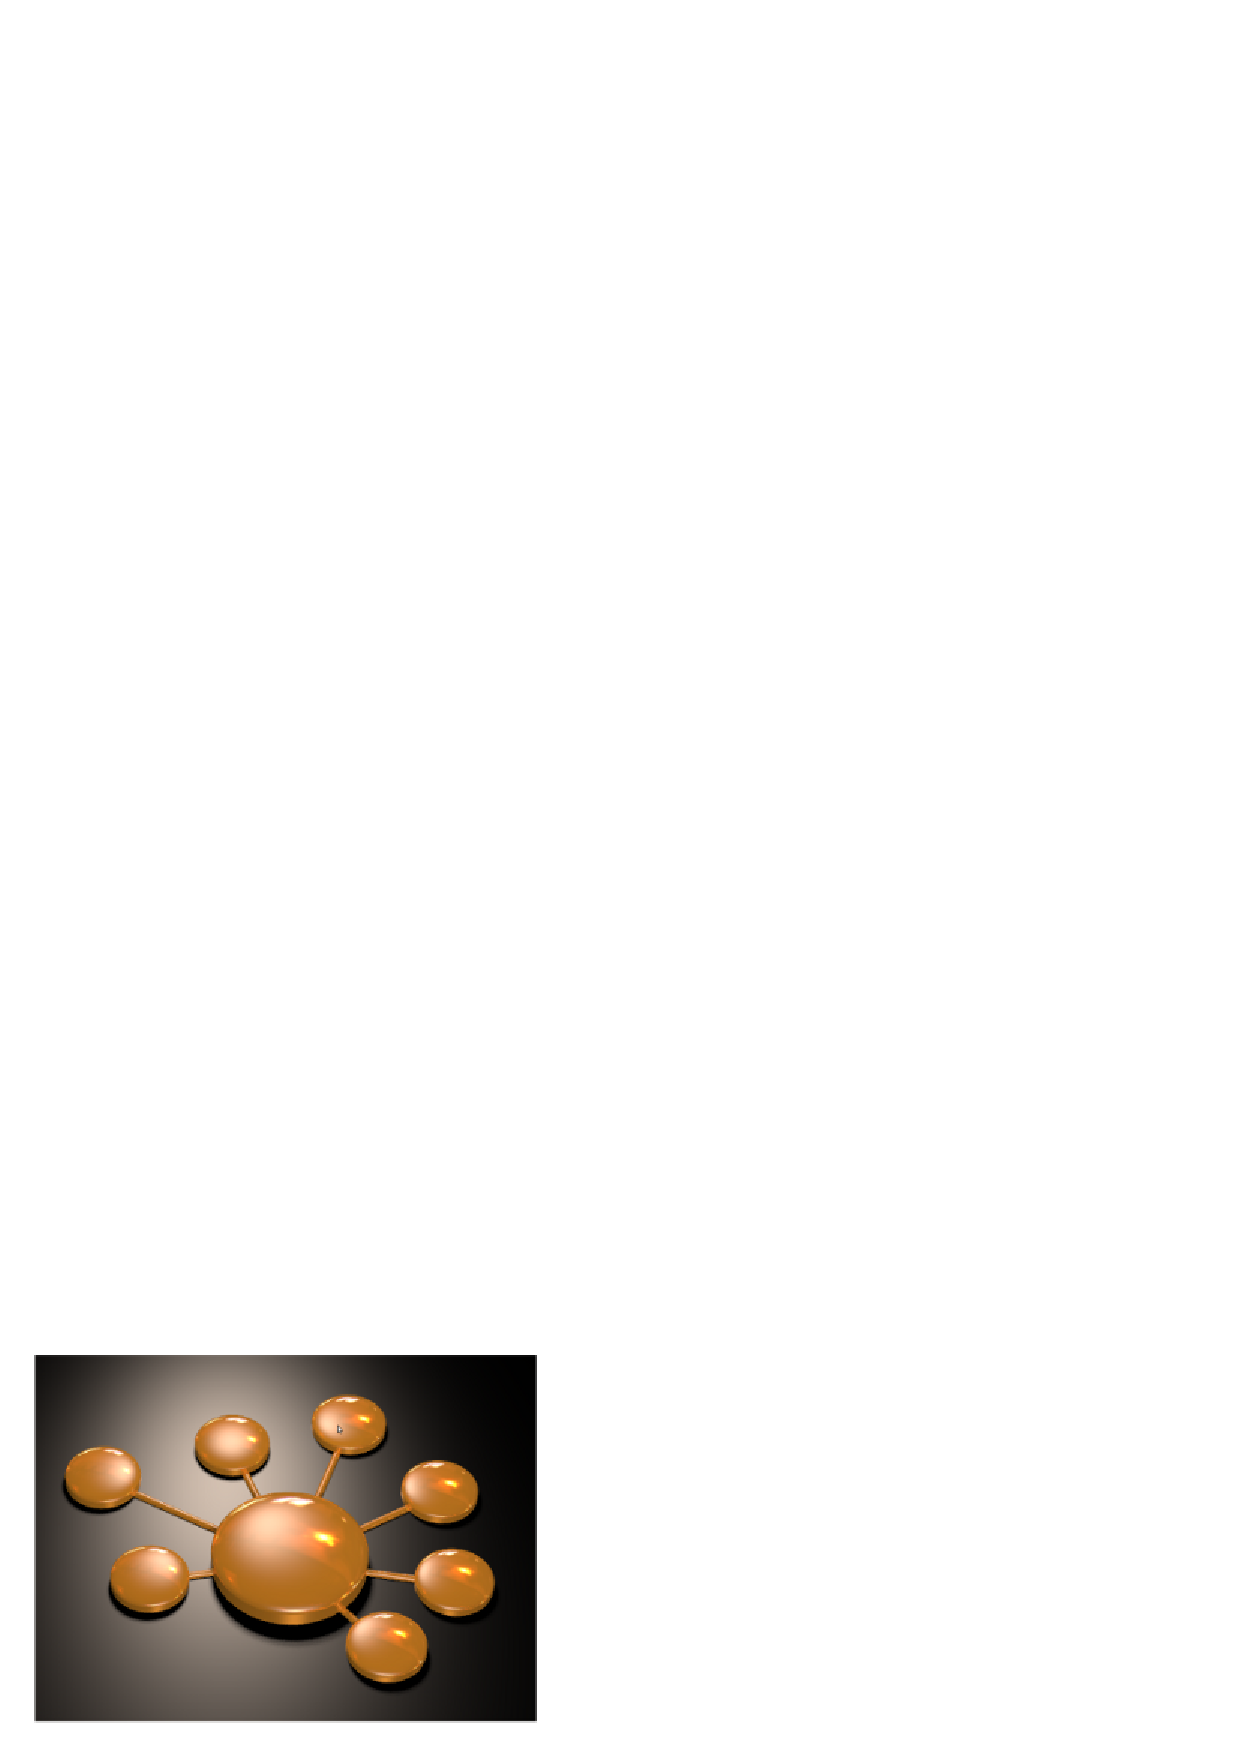
\includegraphics[scale=0.3]{SoFa_Logo}}}
\rput(-4,1.5){\href{http://www.sofa-framework.org/}{
		\begin{tabular}{l}
		\resizebox{4cm}{0.6cm}{SOFA} \\ 
		\resizebox{6cm}{0.3cm}{Simulation Open Framework Architecture}
		\end{tabular}
		}
	    }
\end{center}
%%%%%%%%%%%%%%%%%%   LOGO  %%%%%%%%%%%%%%%%%%%%%%%%%

%%%%%%%%%%%%%%%%%% DOCUMENT TITLE %%%%%%%%%%%%%%%%%%%%%%%%% To be deleted when include in the global document
%\chapter{Mapping} %\section{Rigid Mapping} 
\vspace{1.5cm}
\begin{center}\resizebox{7cm}{0.6cm}{Linear Solver}\end{center}
%%%%%%%%%%%%%%%%%% DOCUMENT TITLE %%%%%%%%%%%%%%%%%%%%%%%%%

%%%%%%%%%%%%%%%%%%%%%%%%%%%%%%%%%%%%%%%%%%%%%%%%%%%%%%%%%%%%%%%%%%%%%%%%%%%%%%%%%%%%%%%%%
%=======================================================================================%
%%%%%%%%%%%%%%%%%%%%%%%%%%%%%%%%%%%%%%%%%%%%%%%%%%%%%%%%%%%%%%%%%%%%%%%%%%%%%%%%%%%%%%%%%
%\section{Linear Solver}% for adding to the global document of SOFA

\section{Linear Solver}
\paragraph{Abstract : }
%%%%%%%%%%%%%%%%%%   LOGO  %%%%%%%%%%%%%%%%%%%%%%%%%
%%%%%%%%%%%%%%%%%%   LOGO  %%%%%%%%%%%%%%%%%%%%%%%%%
In SOFA, all states of a mechanical object is described by its degree of freedom. The main works for the simulation are filling and inverting a matrix system in order to find the states of mechanical objects by steps of time. This system matrix can be described as below :
 \[
\left[ \textbf{MBK} \right].a=f \text{    ,  or at time n+1 :   }\left[ \textbf{MBK} \right].a_{n+1}=f_{n+1}
\]
where,
\[
\left\{ 
\begin{array}{l}
\textbf{M} \text { : the mass matrix   }  \\
\textbf{B} \text { : the damping matrix   }  \\
\textbf{K} \text { : the stiffness matrix   }  \\
\left[ \textbf{MBK} \right] \text {  : is a linear combination of MBK (not multiplication)   }  \\
a_{n+1} \text { : accelerator field} \\
f_{n+1} \text { : force field} 
\end{array}\right.
\]
 Usually, \textbf{M} is filled by \textbf{\color{orange}mass} components, \textbf{K} is filled by \textbf{\color{orange}forcefield} or \textbf{\color{orange}interactionforcefield} components, \textbf{B} (often $\alpha\textbf{M}+\beta\textbf{K}$ ) and $\left[ \textbf{MBK} \right]$ are computed by \textbf{\color{orange}odesolver} components. The works left to invert the matrix system are done by \textbf{\color{orange}linearsolver} components.
\begin{center}
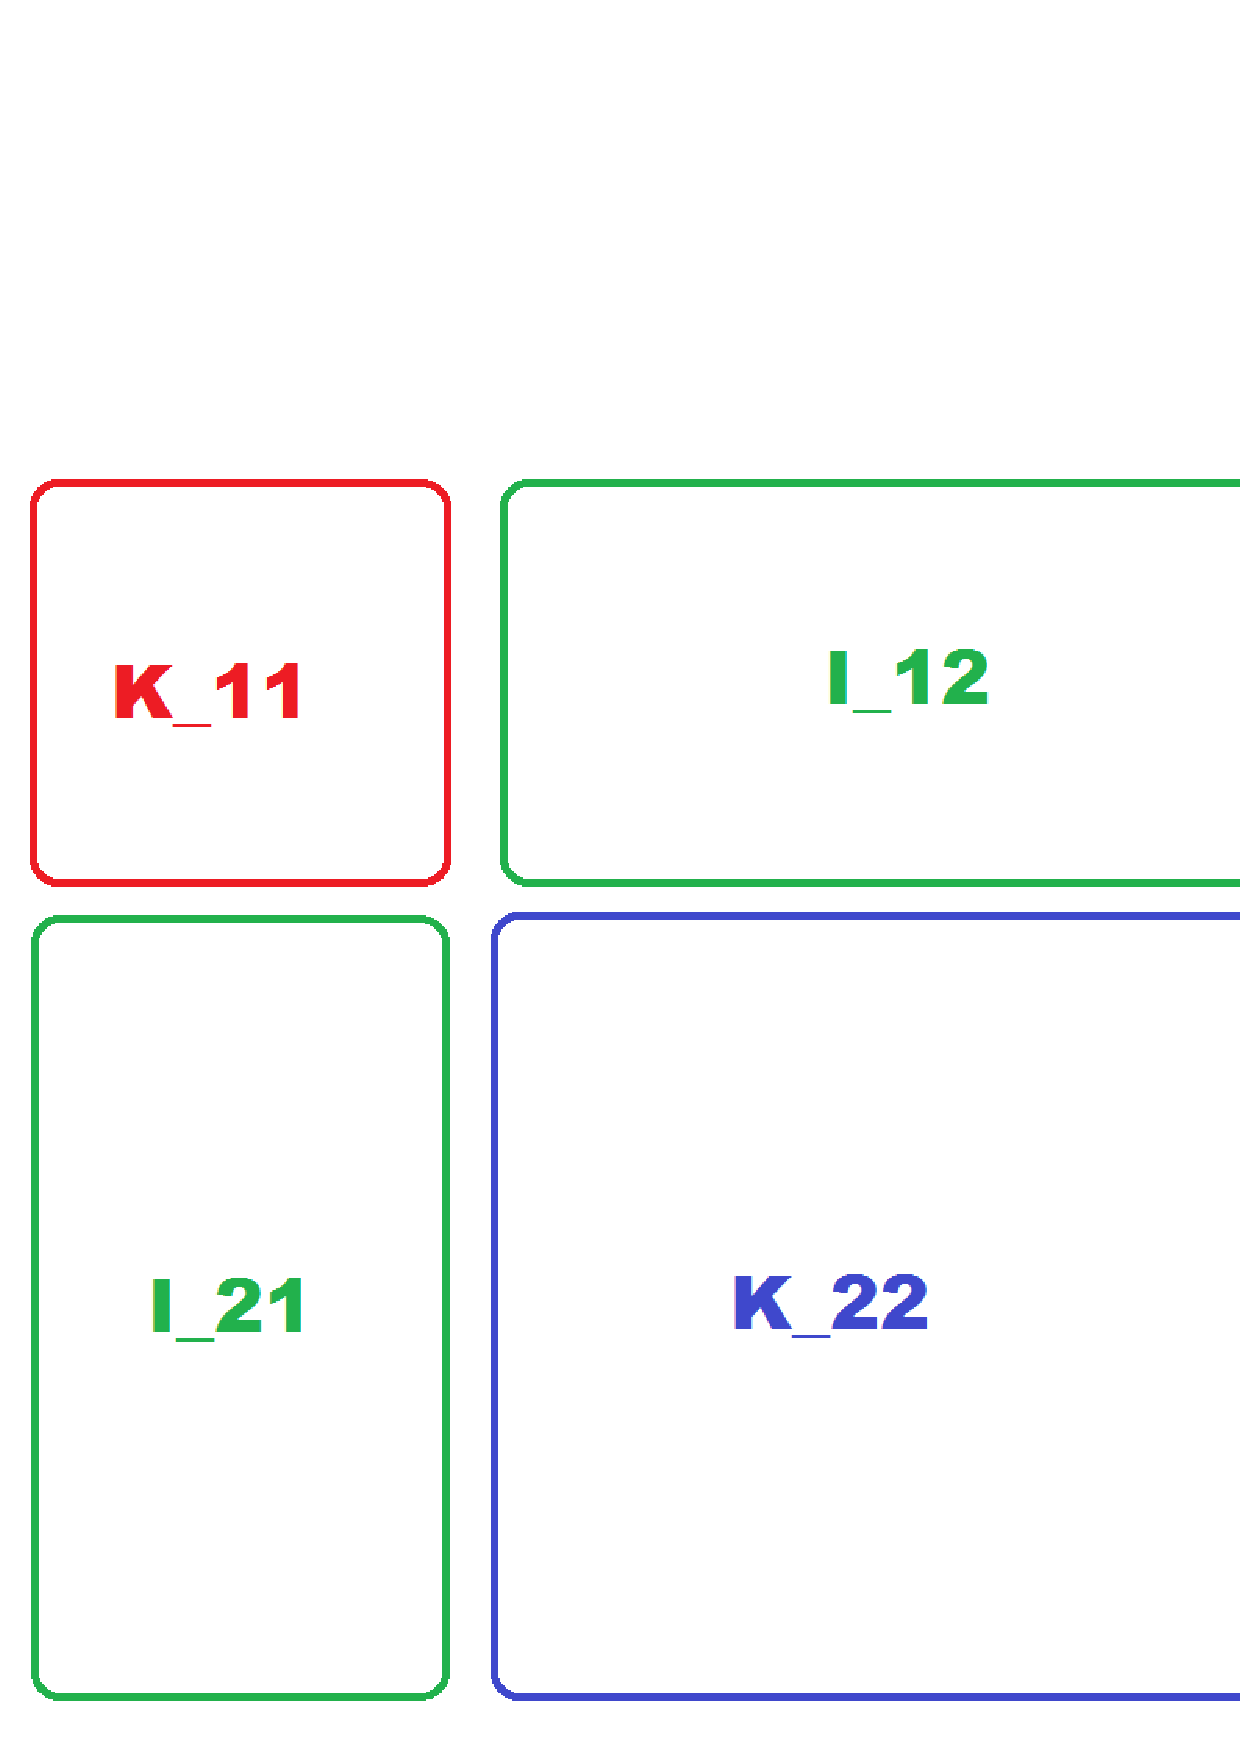
\includegraphics[scale=0.3]{matrix_bloc}
\end{center}
On the case for example when there are two mechanical objects, we can see a global stiffness matrix describing the two mechanical states, composed diagonal blocs and non-diagonal blocs. The diagonal blocs are filled by \textbf{\color{orange}mass},\textbf{\color{orange}forcefield} components, and the non-diagonal ones are filled by \textbf{\color{orange}interactionforcefield} if existed.
\paragraph{Mapping matrix contribution : } When existe a mapping on the simulation scene, the states of two mechanical objects are relied by : 
\[
\begin{array}{rl}
\textbf{x}_{2} & = \Im\left(\textbf{x}_{1}\right)           \text{      ,	mapping::apply}             \\
\textbf{v}_{2} & = \left[\textbf{J}\right] \textbf{v}_{1}   \text{      ,	mapping::applyJ}  
\end{array}
\]
The $\left[\textbf{J}\right]$ matrix is derivative of $\Im$ operator and is defined by the \textbf{\color{orange}mapping} components. The dynamic and matrix system of the two objects are relied by :   
\[
\begin{array}{rl}
\textbf{f}                  & += \textbf{f}_{1}  +   \left[\textbf{J}\right]^{t} \textbf{f}_{2}         \text{      ,	mapping::applyJT}             \\
\left[ \textbf{MBK} \right] & += \left[ \textbf{MBK} \right]_{1}  + \left[\textbf{J}\right]^{t}  \left[ \textbf{MBK} \right]_{2} \left[\textbf{J}\right]
\end{array}
\]
The resolution of the system with the mapping is done in general :
\[
\left\{ 
\begin{array}{rl}
\textbf{a}^{n+1}        & = \left[ \textbf{MBK} \right]^{-1}  \textbf{f}^{n+1}    \\
\textbf{v}^{n+1}_{1}    & = \textbf{v}^{n}_{1}     + dt.\textbf{a}^{n+1}         \\
\textbf{x}^{n+1}_{1}    & = \textbf{x}^{n}_{1}     + dt.\textbf{v}^{n+1}         \\
\textbf{x}^{n+1}_{2}    &  \text{ ,	mapping::apply }     \\
\textbf{v}^{n+1}_{2}    &  \text{ ,	mapping::applyJ }          
\end{array}
\right.
\]



\subsection{Direct Solvers }
The direct solver demande to build explicitly the matrix, and invert this matrix after every step of time in order to solve the mechanical response after a sollicitation.
\subsection{Context in SOFA }
In SOFA, there are a litle more complicated component called mapping, relying geometrical and mechanical propreties by master-slave (DOF-mapped object) relation. All changes of geometry or sollicitation to one object interfere to other and vice versa. If the mapped object have its own mechanical behavior, it must be counted on the mechanical propagation by the mapping.
\subsubsection{self-stiffness propagation }
\[
\begin{array}{cc}
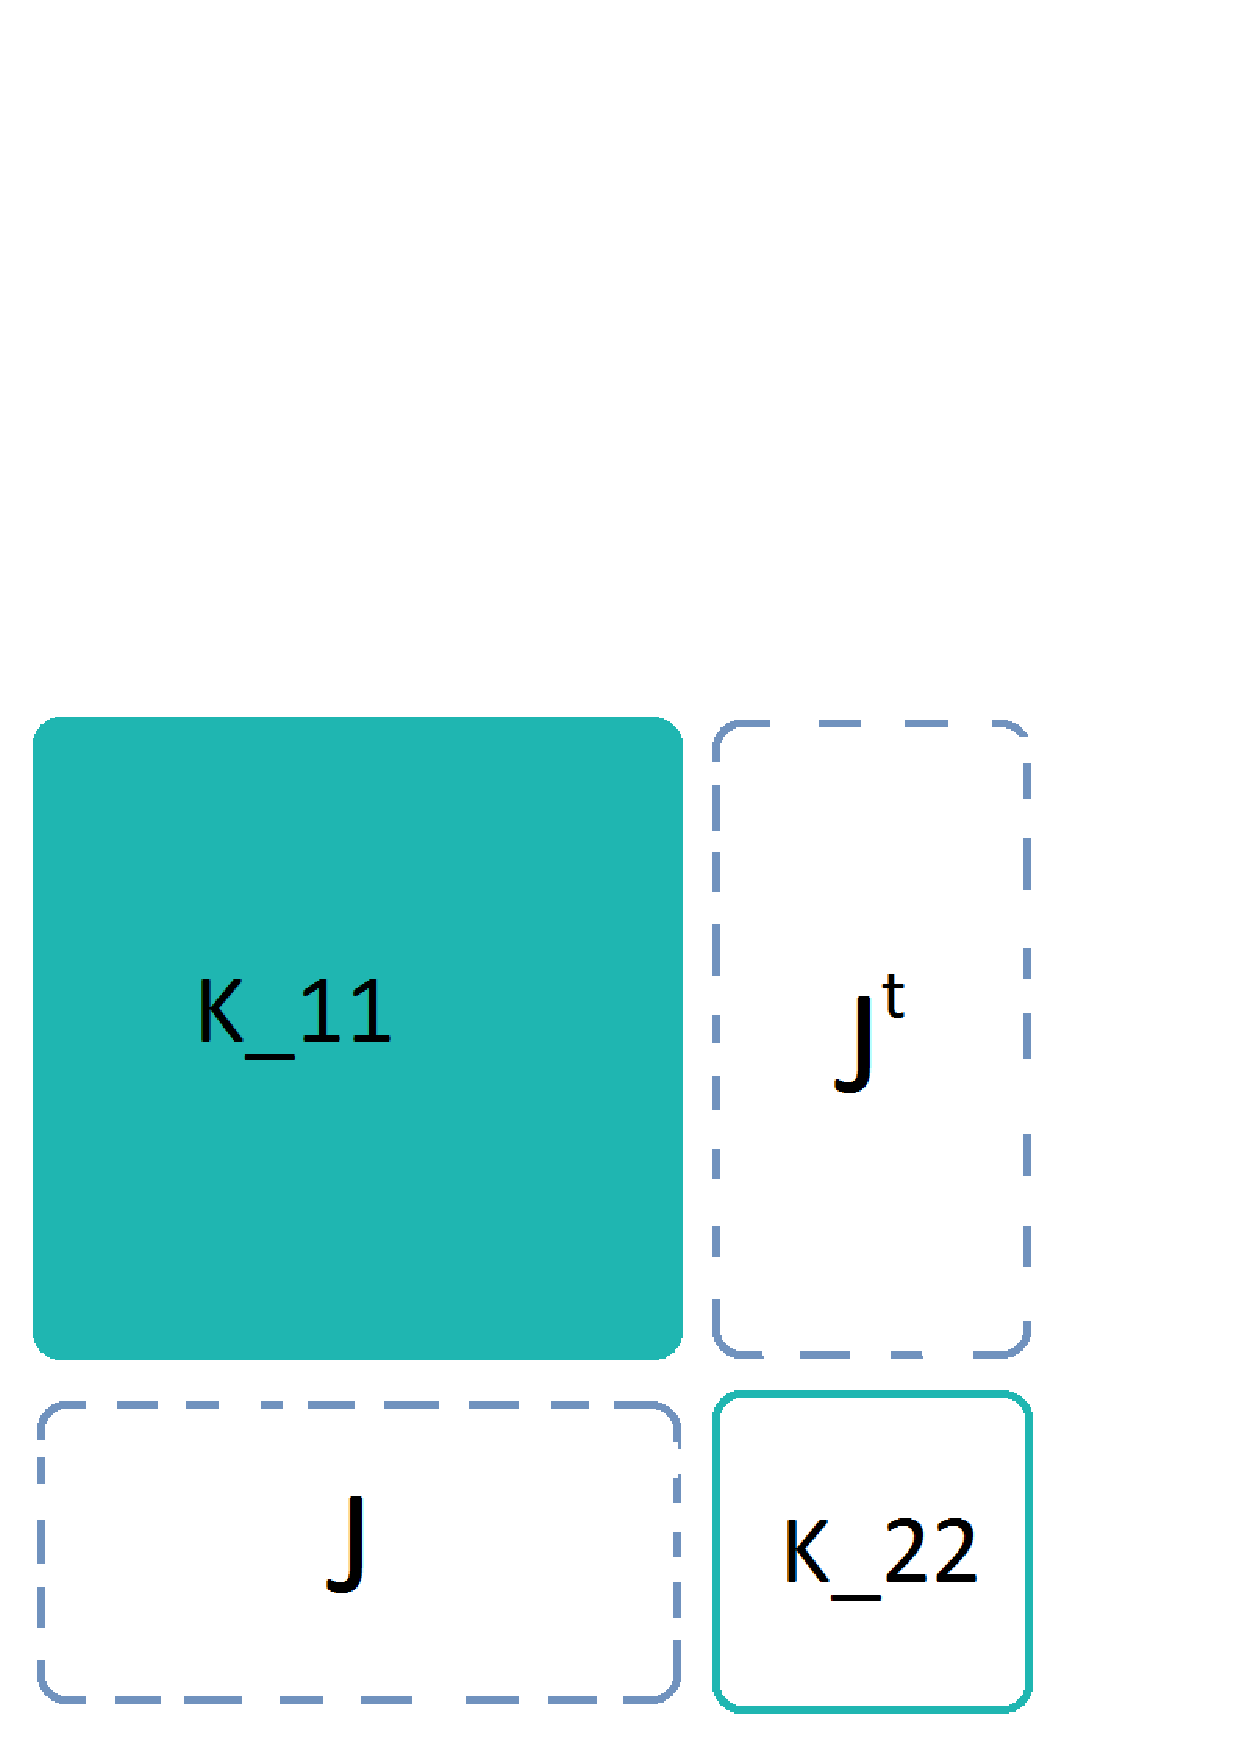
\includegraphics[scale=0.3]{stiffness_propagation_matrix}        
& 
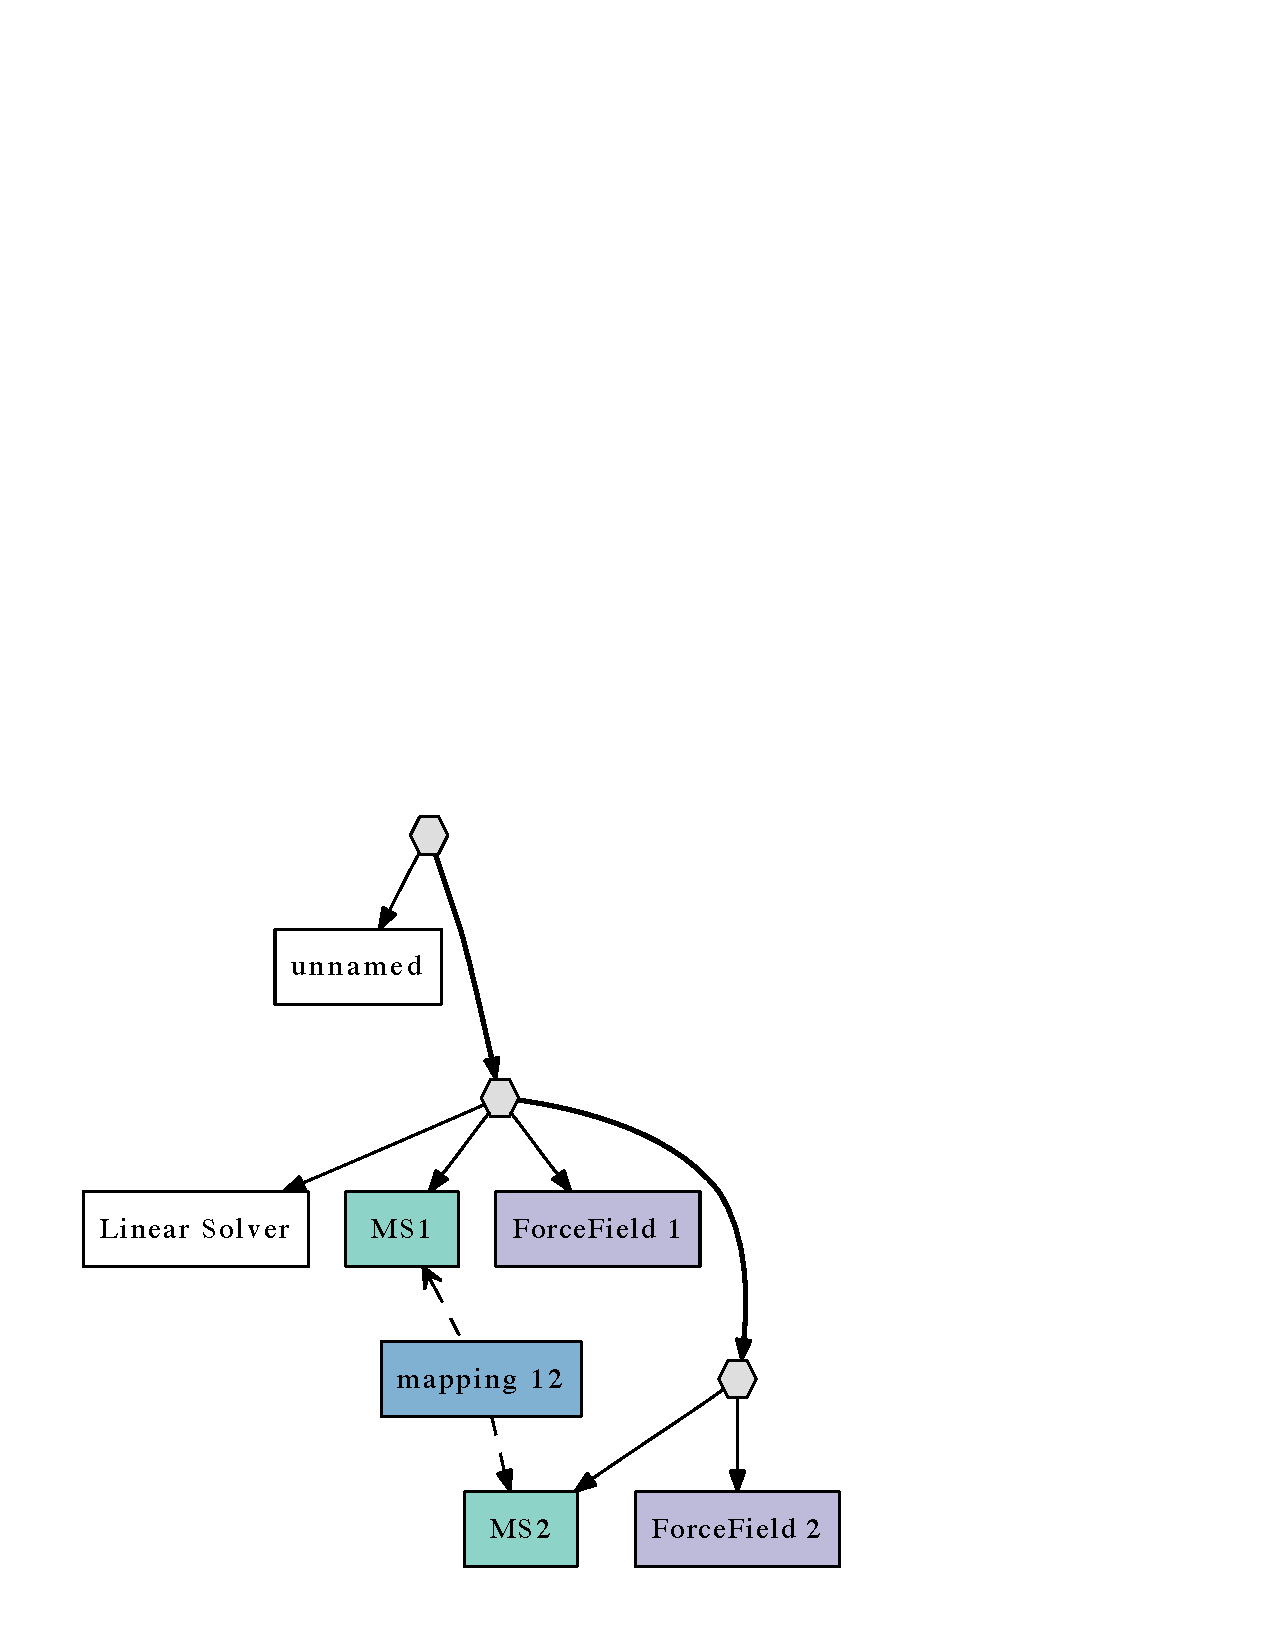
\includegraphics[scale=0.35]{stiffness_propagation} 
\end{array}
\]
In the simple simulation scene, \textbf{MS2} is a mapped object to the \textbf{MS1} mechanical object by the mapping. The matrix to be inverted for all mechanical response is the filled colorized one ($K_{11}$), the matrix $K_{22}$ describing mechanical propreties of the second objects must contribute to $K_{11}$ by the formula :
\[
\left\{ 
\begin{array}{ll}
K_{11}       & += J^t * K_{22} * J               \\
\text{or,}   &         \\
K_{tempo}    & =  J^t * K_{22}                   \\
K_{11}       & += K_{tempo} * J                  \\         
\end{array}
\right.
\]
By doing this computation, we propagate the stiffness of the mapped mechanical object to its root mechanical object.
\subsubsection{interaction-stiffness propagation }
In the general case, the may have a simulation scene where there are many level of mapped mechanical states (mapped of mapped state ...) and many interaction forcefield interacting beetween them. Therefor the stiffness of interaction forcefield and the mapped mechanical state need to be propagated through the mappings. We can imagine for one propagation, there are two simple cases.
\paragraph{Interaction beweent Real Mechanical Object and Mapped Mechanical Object}
\[
\begin{array}{cc}
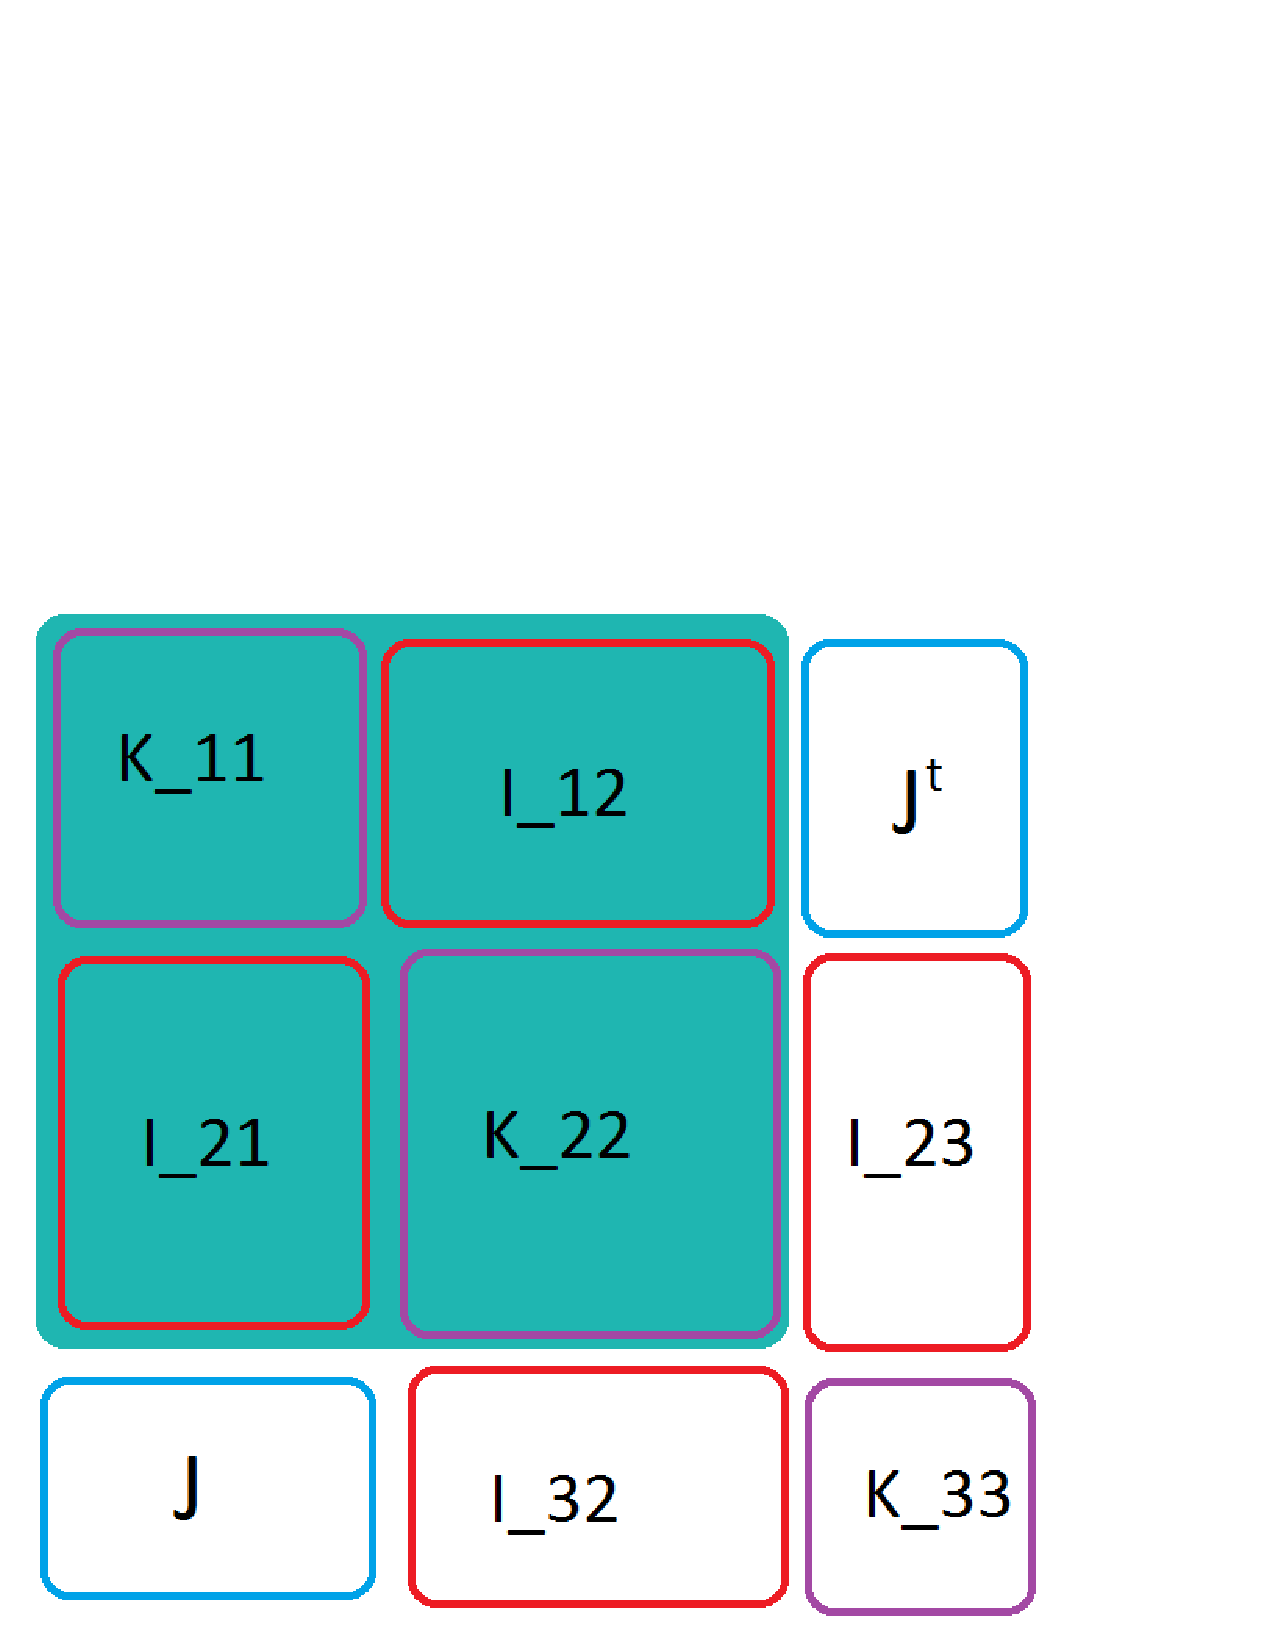
\includegraphics[scale=0.3]{interaction_Real_Mapped_Matrix}        
& 
\includegraphics[scale=0.35]{interaction_Real_Mapped} 
\end{array}
\]
In the case where one of the two mechanical states in interaction is non-mapped, the propagation can be computed directly by the formula :
\[
\left\{ 
\begin{array}{ll}
K_{11}       & += J^t * K_{33} * J               \\
\text{or,}   &                                   \\
K_{tempo}    & =  J^t * K_{33}                   \\
K_{11}       & += K_{tempo} * J                  \\ 
\text{and,}&                 \\      
I_{12}       & += J^t * I_{32}                   \\ 
I_{21}       & += I_{23} * J                        
\end{array}
\right.
\]
\paragraph{Interaction beweent Mapped Mechanical Object and Mapped Mechanical Object}
\begin{center}
  \includegraphics[scale=0.3]{interaction_Mapped_Mapped}
\end{center}
In the case where the two mechanical states in interaction are mapped, the propagation can be computed by two steps. The first consist to propagate the interaction $I_{34}$ to the interation $I_{14}$ :
\[
\left\{ 
\begin{array}{ll}
K_{11}       & += J^t * K_{33} * J               \\
\text{or,}   &                                   \\
K_{tempo}    & =  J^t * K_{33}                   \\
K_{11}       & += K_{tempo} * J                  \\ 
\text{and,}&                 \\      
I_{14}       & += J^t_A * I_{34}                  \\ 
I_{41}       & += I_{43} * J_A                        
\end{array}
\right.
\]
The following step can compute as the one of above paragraph, propagating the interation $I_{14}$ to $I_{12}$.
\subsection{Iterative Solvers }
\subsection{Preconditioner }



						      %%%%%%%%%%%%%%%%%%%%%%%%%%  Writer %%%%%%%%%%%%%%%%%%%%%%%%
						      \begin{flushright}
						      Document written by \\
						      \href{mailto:chi-thanh.nguyen@inria.fr}{{\textbf {Chi Thanh NGUYEN}}} \\
						      INRIA Lille
						      \end{flushright}
						      %%%%%%%%%%%%%%%%%%%%%%%%%%  Writer %%%%%%%%%%%%%%%%%%%%%%%%

%\bibliographystyle{siam}
%\bibliography{mybiblio}
\end{document}
